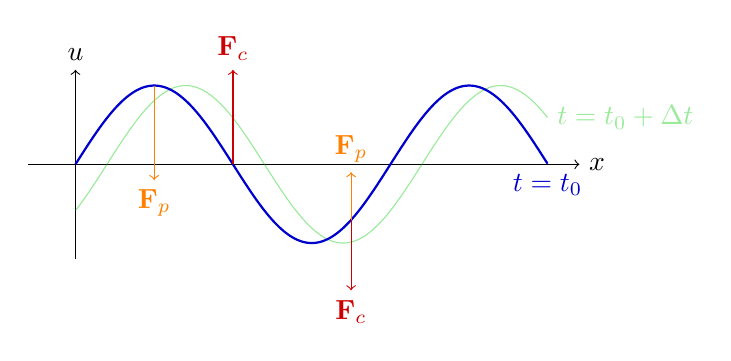
\begin{tikzpicture}[xscale = 2]
\draw[->] (-0.3, 0) -- (3.2,0) node[right] {$x$};
\draw[->] (0, -1.2) -- (0, 1.2) node[above] {$u$};

\draw[green!80!black, opacity = 0.4, domain = 0:3, variable = \x, samples = 300] plot[smooth] ({\x}, {sin((pi * (\x - 0.2)) r)}) node[right] {$t = t_0 + \Delta t$};
\draw[thick, blue!80!black, domain = 0:3, variable = \x, samples = 300] plot[smooth] ({\x}, {sin((pi * \x) r)}) node[below] {$t = t_0$};

\draw[red!80!black, ->] (1, 0) -- (1, 1.2) node[above] {$\mathbf{F}_c$};
\draw[orange, ->] (0.5, 1) -- (0.5, -0.2) node[below] {$\mathbf{F}_p$};
\draw[orange, ->] (1.75, {sin(1.75 * pi r)}) -- (1.75, -0.1) node[above] {$\mathbf{F}_p$};
\draw[red!80!black, ->] (1.75, {sin(1.75 * pi r)}) -- (1.75, -1.6) node[below] {$\mathbf{F}_c$};
\end{tikzpicture}
